\chapter{Limits and colimits}

We've seen pairs in the internal language, but what about record types?
For instance,
\[
\mathsf{Point} = \{
x: \R, y: \R, z: \R
\}
\]
This leads to the idea of indexed products.
\begin{definition}
  \sloppy
  Let \((X_i)_{i\in I}\) be an \(I\)-indexed
  family of objects of a category \(\calC\).
  An \emph{indexed product} of \((X_i)_{i\in I}\)
  consists of an object \(P\)
  and a family of morphisms \((\pi_i : P \to X_i)_{i\in I}\)
  satisfying the following universal property:
  for any object \(Y\)
  and any family of morphisms \((f_i : Y \to X_i)_{i\in I}\),
  there exists a unique morphism \(\angled{f_i}_{i\in I} : Y \to P\)
  such that \(\pi_i \circ \angled{f_i}_{i\in I} = f_i\) for all \(i\) in \(I\).
\end{definition}
While records are typically finite, the definition of indexed product
works just as well for infinite products.
For example,
\begin{proposition}
  \(1\) is the indexed product of \((k)_{k\in \N}\)
  in the category of natural numbers under divisibility.
\end{proposition}
More generally, indexed products in preorders are like infima.

Indexed products are in some sense the ``largest'' way to map
into a collection of objects.
For example, the product for \(\mathsf{Point}\)
is the ``largest'' way of filling in the question marks in this diagram:
\[% https://tikzcd.yichuanshen.de/#N4Igdg9gJgpgziAXAbVABwnAlgFyxMJZABgBoBGAXVJADcBDAGwFcYkQAdDgJRAF9S6TLnyEU5CtTpNW7LrwFDseAkQBMkmgxZtEnHv0EgMy0UQnEp22XoD8-KTCgBzeEVAAzAE4QAtkgBmGhwIJDJpHXZ7GkZ6ACMYRgAFYRUxEC8sZwALHENPH39EIJAQpAkImxB7RRBvP0Dg0MQNSt1qhz4gA
\begin{tikzcd}
   & ? \arrow[ld, "?"'] \arrow[d, "?"] \arrow[rd, "?"] &    \\
\R & \R                                                & \R
\end{tikzcd}\]
Similarly, \(1\) is the ``largest'' way to fill in
the question marks in this diagram:
\[% https://tikzcd.yichuanshen.de/#N4Igdg9gJgpgziAXAbVABwnAlgFyxMJZARgBpiBdUkANwEMAbAVxiRAH4QBfU9TXfIRQAGUsKq1GLNsW68QGbHgJEy46vWatEIAExy+SwUV1iJm6ToDMBhf2VDkVsxqnaQAHQ9QIOBFwkYKABzeCJQADMAJwgAWyRREBwIJDJJLTZOHkiY+MRE5KRTdMsOW2i4hOpCxGcS9yz5CryClMQAFlcMnU5qBjoAIxgGAAV7Yx0orGCACxxuCi4gA
\begin{tikzcd}
1 & 2                                                                  & 3 & \dots \\
  & ? \arrow[lu, "?"] \arrow[u, "?"] \arrow[ru, "?"] \arrow[rru, "?"'] &   &
\end{tikzcd}\]

All of these diagrams are ``discrete'': they consist only of objects,
with no morphisms connecting them.
More generally, we can ask if it is possible to find the largest
way of mapping into an arbitrary diagram consisting of both objects and morphisms.
This is called a \emph{limit}.

We have seen two examples of limits already, in the homework.
\begin{itemize}
\item Given two morphisms \(X \mor{f} Z \xleftarrow{g} Y\),
  the \emph{pullback} is the largest way of mapping into \(f,g\),
  in other words the largest way of filling in the question marks in this
  diagram:
  \[
  % https://tikzcd.yichuanshen.de/#N4Igdg9gJgpgziAXAbVABwnAlgFyxMJZABgBoBGAXVJADcBDAGwFcYkQANEAX1PU1z5CKcqWLU6TVuwCaPPiAzY8BIqKo0GLNohAAtef2VCiZcZqk6QAfh4SYUAObwioAGYAnCAFskAZhocCCQySW12WxpGegAjGEYABQEVYRAPLEcACxxDEE8ff0DgxFEw6V1bXncvXxKipAAmC3DdR1z82tCgxubyvJAo2Pik41VddKyc7kpuIA
\begin{tikzcd}
? \arrow[d, "?"'] \arrow[r, "?"] & Y \arrow[d, "g"] \\
X \arrow[r, "f"']                & Z
\end{tikzcd}
  \]
  Explicitly, a pullback is a 3-tuple \((W,p,q)\)
  where \(p : W \to X\) and \(q : W \to Y\)
  and \(fp = gq\)
  satisfying the following universal property:
  for any other 3-tuple \((W',p',q')\)
  where \(p' : W' \to X\) and \(q' : W' \to Y\)
  and \(fp' = gq'\),
  there exists a unique morphism \(w : W' \to W\)
  such that \(pw = p'\) and \(qw = q'\).
  \[% https://tikzcd.yichuanshen.de/#N4Igdg9gJgpgziAXAbVABwnAlgFyxMJZARgBoAmAXVJADcBDAGwFcYkQANEAX1PU1z5CKcqWLU6TVuwCaPPiAzY8BIqKo0GLNohAAtef2VCiZcZqk6QAdUOKBK4cgAMpZxK3Td1gOQ8JMFAA5vBEoABmAE4QALZIAMw0OBBIrpLa7GggNIz0AEYwjAAKDia6kVhBABY4dlGxCUkpiGTpXiAAjnXRcS1NSKJtVkHdDYhpyQMWGbrh2SC5BcWlquWVNaO9ACz94zQFYFBIALTxaZ5WXTn5hSXGqyAV1bW8ET1IOyCTfSAHR4hnabtDp+V4gerbXaJIbsADu-m4QA
\begin{tikzcd}
W' \arrow[rdd, "q"', bend right] \arrow[rrd, "q'", bend left] \arrow[rd, "w"] &                                  &                  \\
                                                                              & W \arrow[d, "p"'] \arrow[r, "q"] & Y \arrow[d, "g"] \\
                                                                              & X \arrow[r, "f"']                & Z
\end{tikzcd}\]
\item Given two morphisms \(% https://tikzcd.yichuanshen.de/#N4Igdg9gJgpgziAXAbVABwnAlgFyxMJZABgBpiBdUkANwEMAbAVxiRAA0QBfU9TXfIRQBGclVqMWbAJrdxMKAHN4RUADMAThAC2SMiBwQkokHAAWWNTmPV6zVohCKQ1BnQBGMBgAV+eAmwaWIpm1jzqWrqI+oY2EvZsai6mFlZIALTCXBRcQA
\begin{tikzcd}
X \arrow[r, "g"', shift right] \arrow[r, "f", shift left] & Y
\end{tikzcd}\),
their \emph{equalizer} is the largest way of mapping into \(f,g\)
in other words the largest way of filling in the questino marks in this
diagram:
\[% https://tikzcd.yichuanshen.de/#N4Igdg9gJgpgziAXAbVABwnAlgFyxMJZABgBoBGAXVJADcBDAGwFcYkQANEAX1PU1z5CKAEwVqdJq3YBNHnxAZseAkXKliEhizaIQAfh4SYUAObwioAGYAnCAFskZEDghJ1IOAAssVnO5ptaT1TEBpGegAjGEYABQEVYRAbLFMvf15rO0dEZ1cAyR12KzDPHz8kAFpyTJBbByQxFzdcwKldA1KI6LiEoXYUtIyFepym-MQPII7DbkpuIA
\begin{tikzcd}
                                                            & ? \arrow[ld, "?"'] \arrow[rd, "?"] &   \\
X \arrow[rr, "g"', shift right] \arrow[rr, "f", shift left] &                                    & Y
\end{tikzcd}\]
Explicitly, the equalizer is a 3-tuple \((W,p,q)\)
where \(p : W \to X\) and \(q : W \to Y\)
and \(fp = q\) and \(gp = q\)
satisfying the following universal property:
for any other 3-tuple \((W',p',q')\)
where \(p' : W' \to X\) and \(q' : W' \to Y\)
and \(fp' = q'\) and \(gp' = q'\)
there exists a unique \(w : W' \to W\)
such that \(pw = p'\) and \(qw = q'\).
\[% https://tikzcd.yichuanshen.de/#N4Igdg9gJgpgziAXAbVABwnAlgFyxMJZABgBoAmAXVJADcBDAGwFcYkQANEAX1PU1z5CKchWp0mrdgE0efEBmx4CRAIylV4hizaIQAdTn8lQtaWJbJugwHIe4mFADm8IqABmAJwgBbJGRAcCCR1EDgACyx3HBCabSk9JxAaRnoAIxhGAAUBZWEQTywncJjeD28-RACg2IkddndksMjopABaVTKQL18kUUDgqrirdjQm1Izs3NM9QuLS+R7K-prEUPjrAEcjboqkAGYaVYCN0bsU9MyckxVZopKmjLAodv3iLqWDo8H1kb1N84gJ4vRBvD57UHfPrDep6ADu9m4QA
\begin{tikzcd}
                                                            & W' \arrow[ldd, "p'"', bend right] \arrow[rdd, "q'", bend left] \arrow[d, "w"] &   \\
                                                            & W \arrow[ld, "p"'] \arrow[rd, "q"]                                            &   \\
X \arrow[rr, "g"', shift right] \arrow[rr, "f", shift left] &                                                                               & Y
\end{tikzcd}\]
This definition can be simplified a bit:
notice that in the 3-tuple \((W,p,q)\),
the morphism \(q\) is forced to be \(fp\).
So it is equivalent to say that an equalizer
is a 2-tuple \((W,p)\)
such that \(fp = gp\),
which satisfies the universal property
that for any other \((W',p')\)
with \(fp' = gp'\), there exists a unique \(w : W' \to W\)
such that \(wp = p'\) and \(wq = q'\).
\[% https://tikzcd.yichuanshen.de/#N4Igdg9gJgpgziAXAbVABwnAlgFyxMJZARgBpiBdUkANwEMAbAVxiRAA0QBfU9TXfIRQAmclVqMWbAJrdeIDNjwEiABjHV6zVohAB1OXyWC1pVeK1TdegOTdxMKAHN4RUADMAThAC2SdSA4EEhkEtps7iDUcAAWWO44SAC0xDwe3n6IAUEhmpI6IE5RILHxiYihDHQARjAMAAr8ykIgnlhOMYlpIF6+SKKBwVl54bpohj0ZSADM1DnDYVYKdt29mbOD-SNLAO7FVbUNTSa6bR1dFFxAA
\begin{tikzcd}
W' \arrow[rd, "p'"] \arrow[d, "w"'] &                                                           &   \\
W \arrow[r, "p"]                    & X \arrow[r, "f", shift left] \arrow[r, "g"', shift right] & Y
\end{tikzcd}\]
\end{itemize}

The equalizer looks like a refinement type:
\[
\text{equalizer of }
\begin{tikzcd}
X \arrow[r, "g"', shift right] \arrow[r, "f", shift left] & Y
\end{tikzcd}
\qquad\leadsto\qquad
\{x : X \mid f(x) = g(x)\}
\]

The pullback looks like a ``fiber product'':
\[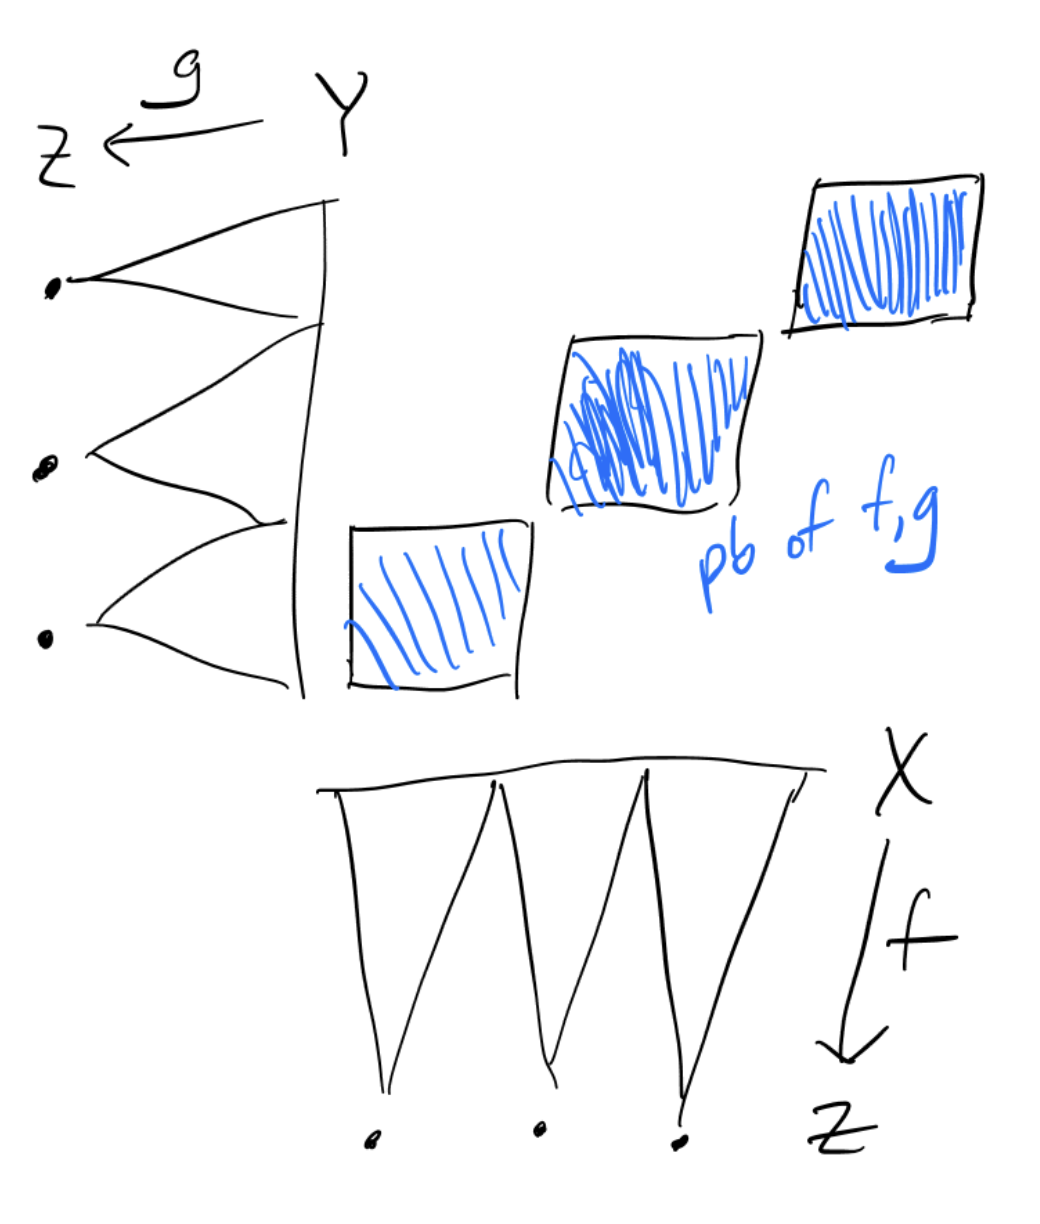
\includegraphics[width=100px]{fig/pb.png}\]

\begin{definition}[cone]
  Let \(D : \mathcal I \to \calC\) be a diagram of shape \(\mathcal I\)
  in a category \(\calC\).
  A \emph{cone} over \(D\) is a pair \((P,p)\)
  where \(P\) is an object of \(\calC\)
  and \(p\) is a family of morphisms \((p_i : P \to D(i))_{i\in I}\)
  such that \(D(f) \circ p_i = p_j\) for all morphisms \(f : i \to j\)
  of \(\mathcal I\).
\end{definition}

\begin{definition}[limit]
  Let \(D : \mathcal I \to \calC\) be a diagram of shape \(\mathcal I\)
  in a category \(\calC\).
  A \emph{limit} of \(D\) is a terminal cone.
\end{definition}

\subsection{Some important facts}

\begin{proposition}
  Every limit is an equalizer of a product.
\end{proposition}

\begin{proposition}
  The Yoneda embedding preserves limits.
\end{proposition}
